% paper template
\documentclass[10pt,reqno,final]{amsart}
%\documentclass[10pt,reqno,draft]{amsart}

\usepackage{amsmath,amsfonts,amssymb,amsthm}
\usepackage{mathrsfs,version,multirow}
\usepackage{graphicx,fancybox,pifont}
\usepackage{url,hyperref}
\usepackage[notcite,notref]{showkeys}
\usepackage{color}
\usepackage{subfigure}
\usepackage{epstopdf}
\usepackage{cases}
\usepackage{mathtools}
\usepackage{algorithm,algorithmic}
\usepackage{lipsum}

\allowdisplaybreaks

\textheight=21.6cm
\textwidth=15cm
\setlength{\oddsidemargin}{0.5cm}
\setlength{\evensidemargin}{0.5cm}

\renewcommand{\baselinestretch}{1.1}
\renewcommand {\thefootnote}{\fnsymbol{footnote}}

% number of equation, figure and table
\numberwithin{equation}{section}
\numberwithin{figure}{section}
\numberwithin{table}{section}

%======================================================%
%== Command for Equations, Theorems and Lemmas etc. ===%
%======================================================%

\theoremstyle{plain}
\newtheorem{theorem}{Theorem}[section]
\newtheorem{lemma}{Lemma}[section]
\newtheorem{corollary}{Corollary}[section]
%\newtheorem{lemma}[theorem]{Lemma}
%\newtheorem{corollary}[theorem]{Corollary}

\theoremstyle{definition}
\newtheorem{definition}{Definition}[section]
\newtheorem{example}{Example}
\newtheorem{xca}{Exercise}[section]

\theoremstyle{remark}
\newtheorem{remark}{Remark}[section]


% define the new command
\newcommand{\atom}[2]{{\scriptsize\begin{array}{c} #1\\[-1mm] #2 \end{array}}}
\newcommand{\refl}[1]{Lemma~{\rm \ref{#1}}}
\newcommand{\reft}[1]{Theorem~{\rm \ref{#1}}}
\newcommand{\refe}[2]{(\ref{#1})--(\ref{#2})}



\title[Short Title]{This is Full Title}

\author[Author A \; \& \; Author B]{Author A${\,}^{1}$ \quad and \quad Author B${\,}^{2*}$} %$^{\dag}$
%\author{D. Doe, P. T. Frank, and J. E. Smith\thanks{ {\it Email address:} xyz@math.univ.edu.}

\date{\today}

\subjclass[2000]{65L60, 65L05, 65L70}

\keywords{Keyword 1, Keyword 2, error analysis}

\thanks{${}^{*}$Corresponding author (E-mail: xyz@math.univ.edu). The work of this author is
supported in part by ... \\
\indent ${}^{1}$ Department of Computer Science, \LaTeX\ University. \\
\indent ${}^{2}$ Department of Mechanical Engineering, \LaTeX\ University
%Department of Mathematics, Shanghai Normal University, Shanghai 200234,  China
}


\begin{document}

\begin{abstract}
  This is an example \LaTeX\ article. This can be used as a
  template for new articles.  Abstracts must be able to stand alone
  and so cannot contain citations to the paper's references,
  equations, etc.  An abstract must consist of a single paragraph and
  be concise. Because of online formatting, abstracts must appear as
  plain as possible. Any equations should be inline.
\end{abstract}

\maketitle


\section{Introduction}
The introduction introduces the context and summarizes the
manuscript. It is importantly to clearly state the contributions of
this piece of work. The next two paragraphs are text filler,
generated by the \texttt{lipsum} package.
\begin{equation}\label{eq:limite}
  \lim_{n\to\infty}\left(1+\frac{1}{n}\right)^n=e.
\end{equation}

\lipsum[2]

\begin{equation}\label{eq:mulequ}
\left\{\begin{aligned}
&-\Delta u=\cos 3x \sin \pi y, && (x, y) \in G=(0, \pi) \times(0,1), \\
&u(x, 0)=u(x, 1)=0, && 0 \leqslant x \leqslant \pi, \\
&u_{x}(0, y)=u_{x}(\pi, y)=0, && 0 \leqslant y \leqslant 1.
\end{aligned}\right.
\end{equation}
This is an example of quoting an equation \eqref{eq:mulequ}.

%\begin{equation}\label{eq:mulequ2}
%\left\{\begin{array}{ll}
%  -\Delta u=\cos 3x \sin \pi y, & (x, y) \in G=(0, \pi) \times(0,1), \\
%  u(x, 0)=u(x, 1)=0, &  0 \leqslant x \leqslant \pi, \\
%  u_{x}(0, y)=u_{x}(\pi, y)=0, & 0 \leqslant y \leqslant 1.
%\end{array}\right.
%\end{equation}

% The outline is not required, but we show an example here.
The paper is organized as follows. Our main results are in
\ref{sec:main}, our new algorithm is in \ref{sec:alg}, experimental
results are in \ref{sec:experiments}, and the conclusions follow in
\ref{sec:conclusions}.

\section{Main results}
\label{sec:main}

%\subsection{Subsection name}

We interleave text filler with some example theorems and theorem-like
items.

\lipsum[5]

This is a citation example \cite{WoZhMeSh05}.

Here we state our main result as \ref{thm:bigthm}.
%the proof is deferred to \ref{sec:proof}.

\begin{theorem}[$LDL^T$ Factorization \cite{GoVa13}]\label{thm:bigthm}
  If $A \in \mathbb{R}^{n \times n}$ is symmetric and the principal
  submatrix $A(1:k,1:k)$ is nonsingular for $k=1:n-1$, then there
  exists a unit lower triangular matrix $L$ and a diagonal matrix
  \begin{equation*}
    D = \operatorname{diag}(d_1,\dots,d_n),  %\diag(d_1,\dots,d_n)
  \end{equation*}
  such that $A=LDL^T$. The factorization is unique.
\end{theorem}

\lipsum[7]

\begin{theorem}[Mean Value Theorem]\label{thm:mvt}
  Suppose $f$ is a function that is continuous on the closed interval
  $[a,b]$.  and differentiable on the open interval $(a,b)$.
  Then there exists a number $c$ such that $a < c < b$ and
  \begin{equation*}
    f'(c) = \frac{f(b)-f(a)}{b-a}.
  \end{equation*}
  In other words,
  \begin{equation*}
    f(b)-f(a) = f'(c)(b-a).
  \end{equation*}
\end{theorem}

\begin{remark}
Observe that \ref{thm:bigthm}, \ref{thm:mvt} correctly mix references
to multiple labels.
\end{remark}


%Observe that \ref{thm:bigthm,thm:mvt,cor:a} correctly mix references
%to multiple labels.

\begin{corollary}\label{cor:a}
  Let $f(x)$ be continuous and differentiable everywhere. If $f(x)$
  has at least two roots, then $f'(x)$ must have at least one root.
\end{corollary}
\begin{proof}
  Let $a$ and $b$ be two distinct roots of $f$.
  By \ref{thm:mvt}, there exists a number $c$ such that
  \begin{equation*}
    f'(c) = \frac{f(b)-f(a)}{b-a} = \frac{0-0}{b-a} = 0.
  \end{equation*}
\end{proof}

Note that it may require two \LaTeX\ compilations for the proof marks
to show.

Display matrices can be rendered using environments from \texttt{amsmath}:
\begin{equation}\label{eq:matrices}
S=\begin{bmatrix}1&0\\0&0\end{bmatrix}
\quad\text{and}\quad
C=\begin{pmatrix}1&1&0\\1&1&0\\0&0&0\end{pmatrix}.
\end{equation}
Equation \ref{eq:matrices} shows some example matrices.

We calculate the Fr\'{e}chet derivative of $F$ as follows:
\begin{subequations}
\begin{align}
  F'(U,V)(H,K)
  &= \langle R(U,V),H\Sigma V^{T} + U\Sigma K^{T} -
  P(H\Sigma V^{T} + U\Sigma K^{T})\rangle \label{eq:aa} \\
  &= \langle R(U,V),H\Sigma V^{T} + U\Sigma K^{T}\rangle
  \nonumber \\
  &= \langle R(U,V)V\Sigma^{T},H\rangle +
  \langle \Sigma^{T}U^{T}R(U,V),K^{T}\rangle. \label{eq:bb}
\end{align}
\end{subequations}
\ref{eq:aa} is the first line, and \ref{eq:bb} is the last line.

\section{Algorithm}
\label{sec:alg}

\lipsum[40]

\begin{lemma}
  This is lemma environment.
\end{lemma}


\begin{theorem}
  This is theorem environment.
\end{theorem}


Our analysis leads to the algorithm in \ref{alg:buildtree}.

\begin{algorithm}
\caption{Build tree}
\label{alg:buildtree}
\begin{algorithmic}
\STATE{Define $P:=T:=\{ \{1\},\ldots,\{d\}$\}}
\WHILE{$\#P > 1$}
\STATE{Choose $C^\prime\in\mathcal{C}_p(P)$ with $C^\prime := \operatorname{argmin}_{C\in\mathcal{C}_p(P)} \varrho(C)$}
\STATE{Find an optimal partition tree $T_{C^\prime}$ }
\STATE{Update $P := (P{\setminus} C^\prime) \cup \{ \bigcup_{t\in C^\prime} t \}$}
\STATE{Update $T := T \cup \{ \bigcup_{t\in\tau} t : \tau\in T_{C^\prime}{\setminus} \mathcal{L}(T_{C^\prime})\}$}
\ENDWHILE
\RETURN $T$
\end{algorithmic}
\end{algorithm}

\lipsum[41]

\section{Experimental results}
\label{sec:experiments}

\lipsum[45-46]

\begin{example}
  This is example environment.
\end{example}

Figure \ref{fig:a} shows some example results.
%Additional results are available in the supplement in \ref{tab:foo}.

\begin{figure}[htp!]
  \centering
  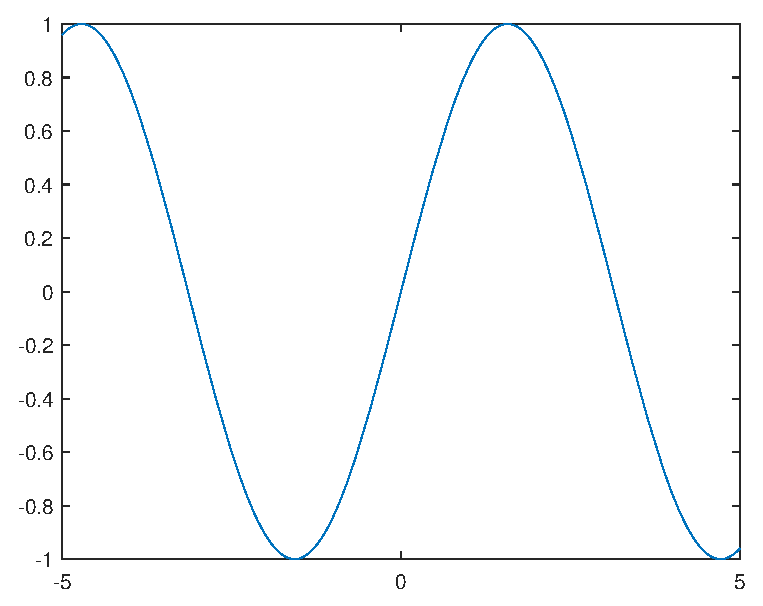
\includegraphics[width=0.48\linewidth]{fig1}
  \caption{Example figure using external image files.}
  \label{fig:a}
\end{figure}

\lipsum[48]

\begin{figure}[htp!]
  \centering
  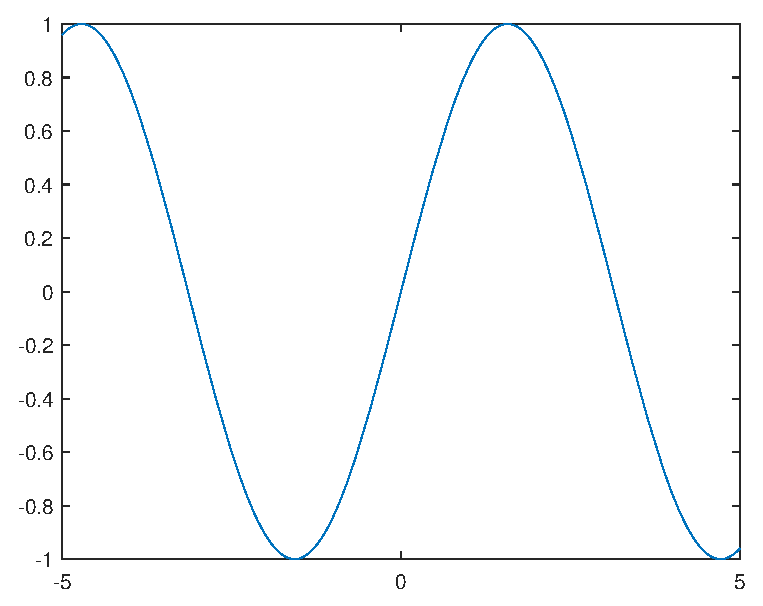
\includegraphics[width=0.48\linewidth]{fig1}
  \hfill
  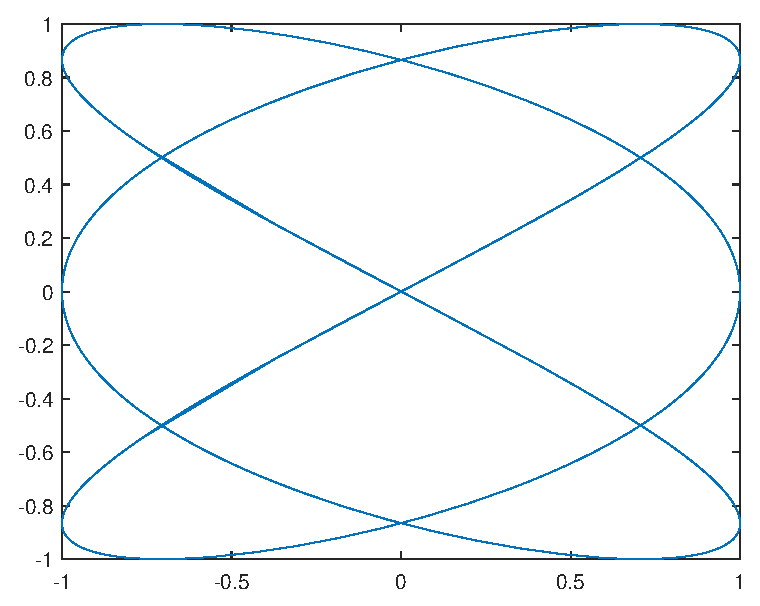
\includegraphics[width=0.48\linewidth]{fig2}
  \caption{Left: Caption 1, Right: Caption 2.}
  \label{fig:b}
\end{figure}


\section{Discussion of \texorpdfstring{{\boldmath$Z=X \cup Y$}}{Z = X union Y}}

\lipsum[76]

\section{Conclusions}
\label{sec:conclusions}

Some conclusions here.


\appendix
\section{An example appendix}
\lipsum[71]

\begin{lemma}
Test Lemma.
\end{lemma}

This is a equation in appendix.
\begin{equation}\label{eq:A1}
  a^2+b^2=c^2.
\end{equation}

\section*{Acknowledgments}
We would like to acknowledge the assistance of volunteers in putting
together this example manuscript and supplement.


\bibliographystyle{plain}
%\bibliographystyle{abbrv}

\bibliography{reference}




\end{document}




